\documentclass[tikz, border=2pt]{standalone}

\usepackage{amsmath,amssymb}
\usepackage{pgfplots}
\pgfplotsset{compat=1.18}
\usetikzlibrary{arrows.meta}
\usepackage{xcolor}

\definecolor{utnblue}{RGB}{0, 51, 102}

\begin{document}
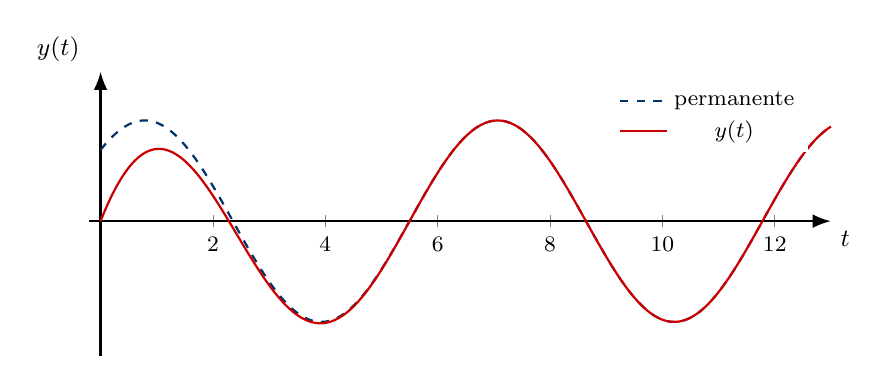
\begin{tikzpicture}[>=Latex, font=\small]
\begin{axis}[
    axis lines=middle,
    axis line style={->, thick, black},
    width=11cm, height=5.2cm,
    xlabel={$t$}, ylabel={$y(t)$},
    xlabel style={anchor=north west},
    ylabel style={rotate=0, anchor=south east, at={(axis description cs:0,1)}},
    xmin=-0.2, xmax=13,
    ymin=-0.95, ymax=1.05,
    ytick=\empty,
    xticklabel style={font=\footnotesize},
    samples=300, domain=0:13,
    clip=false,
    legend style={draw=none, at={(0.97,0.97)}, anchor=north east, font=\footnotesize},
]
    % permanente: (1/sqrt2) cos(t - pi/4) = 0.5 cos t + 0.5 sin t
    \addplot[utnblue, thick, dashed] {0.5*cos(deg(x)) + 0.5*sin(deg(x))};
    \addlegendentry{permanente}
    % salida completa: transitorio -0.5 e^{-t} + permanente
    \addplot[red!80!black, thick] {-0.5*exp(-x) + 0.5*cos(deg(x)) + 0.5*sin(deg(x))};
    \addlegendentry{$y(t)$}
\end{axis}
\end{tikzpicture}
\end{document}
